% Method-Technique

\chapter{Introduction}
\label{ch:introduction}

\chapter{Vector Autoregression}
\label{ch:vector-autoregression}

\textit{Vector autoregressive models (VAR)} is a multivariate
prediction technique where in order to predict a value for each
variable is necessary to take into account the past values of the
variable and of other variables involved in the model. In \textit{VAR}
all variables are interdependent, which means that all variables
depend on the other variables involved in the multivariate system.
This interdependent systems are known in econometric as
\textit{endogenous}.

\textit{VAR} is a generalization of \textit{Autoregressive Models
  (AR)} applied to a vector of time series. Lets analyze the
mathematical expression of a \textit{first order VAR}, or simply
\textit{VAR(1)} for a bivariate system defined in \autoref{eq:var}.

\begin{equation}
  \begin{aligned}
    \label{eq:var}
    y_{1,t} & = c_1 + \phi_{11,1} y_{1,t-1} + \phi_{12,1} y_{2,t-1} +
    e_{1,t} \\
    y_{2,t} & = c_2 + \phi_{21,1} y_{1,t-1} + \phi_{22,1} y_{2,t-1} +
    e_{2,t} 
  \end{aligned}
\end{equation}

In this particular example $y_{i, t}$ describes the variable $i$ in
the temporal instant $t$. This equations define the relationship
between the two variables involved. As the name suggests
\textit{VAR(1)} takes into account only the first lag of each
variable, where $c_i$ is a constant offset and $\phi_{ij,l}$ is the
influence of variable $y_j$ on variable $y_j$ in the $l$-th lag.

\textit{VAR} models need two parameters for fitting. One is the number
of variables, denoted by $K$, and the other one is the number of lags
or $p$. The number of parameters to be estimated in a \textit{VAR} is
$K + p K^2$ or $1 + p K$ per equation. For \autoref{eq:var} there are
two variables, i.e. $K=2$, and only the first lag is used, i.e. $p=1$,
that makes a total of parameters to be estimated of
$2 + 1 \times 2^2 = 6$.

The generalized \textit{VAR(p)} expression would be
\autoref{eq:var-generalized}.

\begin{equation}
  \begin{aligned}
    \label{eq:var-generalized}
    \mathbf{y_t} = \mathbf{c} + \displaystyle\sum_{i=1}^p
    \pmb{\phi_i} \mathbf{y_{t-i}} + \pmb{\epsilon_t}
  \end{aligned}
\end{equation}

If the time series is stationary, we can predict their values by
directly fitting a \textit{VAR} to the data. On the other hand, if the
series is non-stationary we take differences to transform the time
series into a stationary one, and then, fit a \textit{VAR} to the
differenciated data. In both cases the model parameters are estimated
by \textit{OLS} per equation.

The predictions are generated recursively. \textit{VAR} generates a
prediction for each one of the variables involved in the model. Lets
take the \textit{VAR(1)} described in \autoref{eq:var}. \textit{VAR}
would estimate the parameters $\phi_{ij,l}$ and $c_i$ for $y_{i,t}$
such that $i \in \{1,2\}$ and $t = T$. Once the parameters has been
estimated by \textit{OLS} is possible to create the prediction
equations. \autoref{eq:var-prediction-1} describes the prediction
equation for $h=1$

\begin{equation}
  \begin{aligned}
    \label{eq:var-prediction-1}
    \hat{y}_{1,T+1|T} & = \hat{c}_1 + \hat{\phi}_{11,1} y_{1,T} +
    \hat{\phi}_{12,1} y_{2,T} \\ 
    \hat{y}_{2,T+1|T} & = \hat{c}_2 + \hat{\phi}_{21,1} y_{1,T} +
    \hat{\phi}_{22,1} y_{2,T}
  \end{aligned}
\end{equation}

\autoref{eq:var-prediction-1} is very similar to \autoref{eq:var}
except that the parameters has been replaced by its estimated values
and the error has been replaced by zero.

If the horizon we want to use is $h = 2$, the equation would be
\autoref{eq:var-prediction-2} where the values for past values of the
variable are replaced by predictions of those values.

\begin{equation}
  \begin{aligned}
    \label{eq:var-prediction-2}
    \hat{y}_{1,T+2|T} & = \hat{c}_1 + \hat{\phi}_{11,1} \hat{y}_{1,T+1} +
    \hat{\phi}_{12,1} \hat{y}_{2,T+1} \\ 
    \hat{y}_{2,T+2|T} & = \hat{c}_2 + \hat{\phi}_{21,1} \hat{y}_{1,T+1} +
    \hat{\phi}_{22,1} \hat{y}_{2,T+1}
  \end{aligned}
\end{equation}
\chapter{Recurrent Neural Networks}
\label{ch:recurrent-neural-networks}

\section{Artificial Neural Networks}

\textit{Artificial neural networks} are a learning model based on the
human brain's neural network structure. It represents graphically an
ideal structure that resembles that of the neuron and it's connections
with another neurons.

A simple \textit{ANN (artificial neural network)} can be seen in
\autoref{fig:one-layer-ann}. We can see in the first layer, called
\textit{input layer}, the nodes that represent the inputs, represented
as $x_0, x_1, x_2,$ and $x_3$, where $x_1$ through $x_3$ are actual
inputs, and $x_0$ is a \textit{bias term}. This \textit{bias term} is
always equal to 1.

Next we have the directed edges, which represent how the information
flow goes, in this case, the information flows from $x_0, x_1, x_2,
x_3$ to $a_1^{(2)}$, which is in the second layer. In other words,
$a_1^{(2)}$ has $x_0, x_1, x_2, x_3$ as inputs. This edges has
associated weights, which multiply the output of the origin node and
their purpose. In this particular network the weights are represented
by $W_0, W_1, W_2$ and $W_3$. The term $a_1^{(2)}$ means the first
neuron in the second layer. In the next layer, called \textit{output
layer}, we have the output neuron represented by $a_0^{(2)},$
mentioned before. The nodes in this layer have an \textit{activation
function} which can perform different computations with the inputs and
a matrix of weights $W$. In this case is the \textit{sigmoid function}
represented by $\sigma$ with the expression in
\autoref{eq:sigmoid-function}. The expression $h_W(x)$ means that the
output is a parameterized function of the inputs $x$ and that the
parameters are the components of the \textit{weight} matrix $W$.

\begin{figure}[bth]
  \myfloatalign
  {\includegraphics[width=.6\linewidth]
    {gfx/simple-ann-model}}
  \caption{One layer artificial neural network}
  \label{fig:one-layer-ann}
\end{figure}

As you can imagine, the network can have different topologies,
multiple hidden layers, different connection architectures, and
different activation functions. Let's take a look at a two layer
network in \autoref{fig:two-layer-ann}. Just as in
\autoref{fig:one-layer-ann} the first layer is the input layer, with
bias term $x_0$ and inputs $x_1, x_2$ and $x_3$. Next to the input
layer is the hidden layer, which also contains a bias term called
$a_0^{(2)}$ and hidden neurons called $a_1^{(2)}, a_2^{(2)}$ and
$a_3^{(2)}$. In this neural network architecture, called
\textit{multilayer perceptron (MLP)}, each layer is fully connected
with the next, therefore each neuron of the hidden layer except for
the bias term have all the neurons from the input layer as inputs.
Last we have the output layer, which contains a single neuron in
\textit{MLP} called $a_1^{(3)}$. This neuron gives the output of the
neural network which is $h_{W}(x)$.

\begin{figure}[bth]
  \myfloatalign
  {\includegraphics[width=1\linewidth]
    {gfx/two-layer-ann-model}}
  \caption{Two layer artificial neural network}
  \label{fig:two-layer-ann}
\end{figure}

Here we will try to write the relationship between input, output and
the parameters. Let's start by writing the mathematical expression of
the second layer in \autoref{eq:layer-2-expression}. Where
$W_{ik}^{(j)}$ is the weight controlling the mapping between layer $j$
and $j + 1$ for the $k$-th input of the $i$-th neuron in layer $j$,
and $\sigma$ is the activation function.

\begin{equation}
  \begin{aligned}
    \label{eq:layer-2-expression}
    a_1^{(2)} & = \sigma(W_{10}^{(1)} x_0 + W_{11}^{(1)} x_1
    + W_{12}^{(1)} x_2 + W_{13}^{(1)} x_3) \\
    a_2^{(2)} & = \sigma(W_{20}^{(1)} x_0 + W_{21}^{(1)} x_1
    + W_{22}^{(1)} x_2 + W_{23}^{(1)} x_3) \\
    a_3^{(2)} & = \sigma(W_{30}^{(1)} x_0 + W_{31}^{(1)} x_1
    + W_{32}^{(1)} x_2 + W_{33}^{(1)} x_3) \\
  \end{aligned}
\end{equation}

Following with the same procedure we can build the expression for the
output in \autoref{eq:output-expression}.

\begin{equation}
  \begin{aligned}
    \label{eq:output-expression}
    h_{W}(x) & = a_1^{(3)} = \sigma(W_{10}^{(2)} a_0^{(2)}
    + W_{11}^{(2)} a_1^{(2)} + W_{12}^{(2)} a_2^{(2)}
    + W_{13}^{(2)} a_3^{(2)} \\
  \end{aligned}
\end{equation}

We mentioned before the \textit{activation function}. This
\textit{activation function} takes the inputs of the neuron and
outputs a value to the next layer. This value can be a two state value
($\{0,1\}$), or a linear one. In classification the two-state value
are used, and for this outputs the expression that the
\textit{activation function} takes is frequently a \textit{sigmoid
function} or \textit{logistic function}, represented in
\autoref{eq:sigmoid-function}. We have been using a \textit{sigmoid
function} in all our \textit{activation functions}.

\begin{equation}
  \begin{aligned}
    \label{eq:sigmoid-function}
    \sigma(z) = \frac{1}{1 + e^{-z}}
  \end{aligned}
\end{equation}

\section{Backpropagation Algorithm}

\textit{BP} was developed in the context of control theory by
\cite{kelley1960gradient} and later applied to \textit{artificial
intelligence} by \cite{werbos1974beyond} and
\cite{rumelhart1988learning}.

We are going to use gradient descent to optimize the \textit{error
function} in terms of the \textit{weights} of the network. First we
need to find the gradient of the \textit{error function} in with
respect to the \textit{weights}, i.e. $\dfrac{\partial E}{\partial
  W_{ij}^{(l)}}$

In \autoref{eq:sigmoid-function-derivate} we calculate the derivative
of the \textit{sigmoid function} because we are going to use it all
over the \textit{backpropagation} explanation.

\begin{equation}
  \begin{aligned}
    \label{eq:sigmoid-function-derivate}
    \dfrac{d}{dz} \sigma(z) & = \dfrac{d}{dz} \frac{1}{1 + e^{-z}} =
    \dfrac{e^{-z}}{(1 + e^{-z})^2} = \dfrac{1 + e^{-z}}{(1 +
      e^{-z})^2} - \left( \dfrac{1}{1 + e^{-z}} \right)^2 \\
    & = \sigma(z) - (\sigma(z))^2 = \sigma(z)(1-\sigma(z))
  \end{aligned}
\end{equation}

Now let's define the \textit{error function} in
\autoref{eq:error-function}. Let's also define, for the purpose of
this explanation, three disjoint sets of neurons, i.e., the set of
neurons in the input layer which is called $I$ and is indexed by $i$
such as $ i \in I$, the set of neurons in a hidden layer which is
called $J$ and is indexed by $j$ such as $j \in J$, and the set of
neurons in the output layer called $K$ and is indexed by $k$ such as
$k \in K$.

\begin{equation}
  \begin{aligned}
    \label{eq:error-function}
    E = \frac{1}{2} \sum_{k \in K} (h_k - y_k)^2
  \end{aligned}
\end{equation}

To compute the gradient of the \textit{error function} we are going to
compute it for two of the three disjoint sets that we have established
before. Those sets are the \textit{output layer}, and the
\textit{hidden layer}. There's no need to compute the error for the
\textit{input layer} because there isn't an error associated with the
inputs.

In the calculation of the gradient of the output layer in
\autoref{eq:output-layer-error-function-gradient} we have $W_{jk}$
meaning a \textit{weight} between a neuron from the \textit{hidden
layer} to a neuron in the \textit{output layer}, $h_i$, $h_j$ and
$h_k$ are outputs of a neuron in the \textit{input layer},
\textit{hidden layer} or \textit{output layer} respectively.

\begin{equation}
  \begin{aligned}
    \label{eq:output-layer-error-function-gradient}
    \frac{\partial E}{\partial W_{jk}} & = \frac{\partial}{\partial
      W_{jk}} \frac{1}{2} \sum_{k \in K} (h_k - y_k)^2 \\
    & = (h_k - y_k)h_k(1-h_k)h_j \\
    \textbf{substitute } \delta_k & = (h_k - y_k)h_k(1-h_k) \implies \\
    & \implies \frac{\partial E}{\partial W_{jk}} = h_j \delta_k
  \end{aligned}
\end{equation}

Now for a hidden layer, the calculations of the gradient would be the
ones shown in \autoref{eq:hidden-layer-error-function-gradient}.

\begin{equation}
  \begin{aligned}
    \label{eq:hidden-layer-error-function-gradient}
    \frac{\partial E}{\partial W_{ij}} & = \frac{\partial}{\partial
      W_{ij}} \frac{1}{2} \sum_{k \in K} (h_k - y_k)^2 \\
    & = h_j(1-h_j)h_i \sum_{k \in K} (h_k - y_k) h_k(1 - h_k) W_{jk}  \\
    \textbf{substitute } \delta_k & = (h_k - y_k) h_k(1 - h_k) \implies \\
    & \implies \frac{\partial E}{\partial W_{ij}} = h_j(1-h_j)h_i
    \sum_{k \in K} \delta_k W_{jk} \\
    \textbf{substitute } \delta_j & = h_j(1-h_j) \sum_{k \in K} \delta_k
    W_{jk}  \implies \\ 
    & \implies \frac{\partial E}{\partial W_{ij}} = h_i\delta_j
  \end{aligned}
\end{equation}

Once we come up with the gradient results we can present the
backpropagation algorithm in \autoref{backpropagation-algorithm} to
obtain those gradients.

\begin{algorithm}[H]
  \caption{\textit{Backpropagation algorithm}}
  \label{backpropagation-algorithm}
  \begin{algorithmic}[1]
    \State Let the training set be $\{(x^{(1)},y^{(1)}),\dots,
    (x^{(m)},y^{(m)})\}$
    \State Set $\Delta_{ij}^{(l)} = 0$ for all $l,i,j$
    \For{ $i = 1$ to $m$ }
    \State Set $a^{(1)} = x^{(i)}$
    \State Propagate values to compute $a^{(l)}$ for $l = 2,
    3, \dots, L$
    \State Using $y^{(i)}$ compute $\delta^{(L)} = a^{(L)} - y^{(i)}$
    \State Compute $\delta^{(L-1)}, \delta^{(L-2)}, \dots,
    \delta^{(2)}$
    \State $\Delta_{ij}^{(l)} := \Delta_{ij}^{(l)} + a_j^{(l)} \delta_i^{(l+1)}$
    \EndFor
    \State $D_{ij}^{(l)} := \frac{1}{m} \Delta_{ij}^{(l)} + \lambda
    W_{ij}^{(l)}$ if $j \neq 0$
    \State $D_{ij}^{(l)} := \frac{1}{m} \Delta_{ij}^{(l)}$ if $j = 0$
  \end{algorithmic}
\end{algorithm}

In the forward pass, \textit{backpropagation} computes the values of
each neuron until getting the outputs, and in the backward pass,
\textit{backpropagation} computes the error gradients and updates the
\textit{weights} and \textit{biases} of the network.

\section{Recurrent Neural Network}
\label{sec:rnn-nets}

The general idea behind \textit{recurrent neural networks} is the
ability to use information from other elements of a sequence. Thus,
the input of RNNs are considered sequences. Whether they are time
sequences, or notes from a musical composition or words in a sentence,
RNNs can take advantage of this sequential nature of the input.

A \textit{recurrent neural network} (\cite{rumelhart1986sequential})
is a class of artificial neural network where connections between
units form a directed cycle as shown in \autoref{fig:rnn-structure}.
This creates an internal state of the network which allows it to
exhibit dynamic temporal behavior. Unlike feedforward neural networks,
RNNs can use their internal memory to process arbitrary sequences of
inputs. This makes them applicable to tasks such as unsegmented
connected handwriting recognition or speech recognition.

\begin{figure}[bth]
  \centering
  \includegraphics[width=.5\linewidth]{gfx/rnn.png}
  \caption{Recurrent Neural Network}
  \label{fig:rnn-structure}
\end{figure}

The two equations that govern the behavior of this type of neural nets
are described in \autoref{eq:rnn-equations}. This equation

\begin{align}
  \begin{split}
    \label{eq:rnn-equations}
    h^{(t)} & = \sigma(W_{ij} x^{(t)} + W_{jj} h^{(t-1)} + b_h ) \\
    \hat{y}^{(t)} & = \sigma(W_{jk} h^{(t)} + b_y ) \\
    W_{ij} & \gets \text{Matrix of weights between inputs and hidden
      layer} \\
    W_{jj} & \gets \text{Matrix of recurrent weights between hidden
      layer and itself} \\
    b_h, b_y & \gets \text{Biases to learn offsets}
  \end{split}
\end{align}

\section{Backpropagation through time}
\label{sec:bp-through-time}

\textit{Backpropagation through time (BPTT)}, introduced by
\cite{werbos1990backpropagation} is the use of
\textit{backpropagation} over an \textit{RNN}. To be able to apply
\textit{BPTT} there are some issues that must be taken into account.

First the \textit{RNN} need to be unfolded through time in a
\textit{feed forward network (FFN)}. This is done by creating a finite
set of new nodes that represent the same neuron in successive time
steps. This step is performed for every neuron in a \textit{hidden
layer}. This is done because \textit{backpropagation} can't be run
over a network with cycles. \autoref{fig:bptt-unfolded-rnn} shows the
3-step unfolded version of the \textit{RNN} shown in
\autoref{fig:rnn-structure}.

\begin{figure}[bth]
  \centering
  \includegraphics[width=.95\linewidth]{gfx/bptt-unfolded-rnn}
  \caption{Unfolded RNN for BPTT}
  \label{fig:bptt-unfolded-rnn}
\end{figure}

Second, as a consequence of the unfolding, we need to reproduce the
edges connecting those new nodes, so we establish a restriction by
which a set of edges in the \textit{FFN} that are reproduced from one
single edge in the \textit{RNN} need to update their weights by the
same amount. This can be enforced by averaging $\Delta W$ over all the
set each time is computed.
\autoref{fig:bptt-unfolded-rnn-weight-restrictions} shows the weight
restriction that would apply to the unfolded \textit{RNN} of
\autoref{fig:bptt-unfolded-rnn}.

\begin{figure}[bth]
  \centering
  \includegraphics[width=.95\linewidth]
  {gfx/bptt-unfolded-rnn-weight-restrictions}
  \caption{Weight restrictions in unfolded RNN}
  \label{fig:bptt-unfolded-rnn-weight-restrictions}
\end{figure}

%---------------------------------------------------------------------
%---------------------------------------------------------------------
%---------------------------------------------------------------------

%\enlargethispage{2cm}

%------------------------------------------------

%%% Local Variables:
%%% mode: latex
%%% TeX-master: "../main"
%%% End:
